\documentclass[10pt,twocolumn,letterpaper]{article}


\usepackage[review]{cvpr} 
\def\paperID{N/A}
\def\confName{CVPR}
\def\confYear{2026}

\usepackage[table]{xcolor}   % 行列着色
% \usepackage{booktabs}        % \toprule, \midrule, \bottomrule
% \usepackage{graphicx}        % \resizebox
% \usepackage{cancel}
% \usepackage{etoc}     
% \usepackage{tocloft}   
% \usepackage{amsmath, amssymb, amsthm}  % for math 
% \usepackage{bm}  
% \usepackage{booktabs}   % for \toprule, \midrule, \bottomrule
% \usepackage{tabularx}   % for tabularx environment
% \usepackage{array}      % for >{\raggedright\arraybackslash}X
% \usepackage{caption}    
\usepackage{graphicx, cancel, etoc, tocloft, amsmath, amssymb, amsthm, bm, booktabs, tabularx, array, caption, multirow} 
\usepackage[pagebackref,breaklinks,colorlinks,citecolor=cvprblue]{hyperref}

\theoremstyle{plain}
\newtheorem{theorem}{Theorem}
\newtheorem{lemma}{Lemma}
\newtheorem{proposition}{Proposition}
\newtheorem{corollary}{Corollary}

\theoremstyle{definition}
\newtheorem{definition}{Definition}

\theoremstyle{remark}
\newtheorem{remark}{Remark}
% \usepackage[pagebackref,breaklinks,colorlinks,citecolor=cvprblue]{hyperref}
\definecolor{darkgreen}{RGB}{0,128,0}
\definecolor{cvprblue}{rgb}{0.21,0.49,0.74}
\definecolor{lightgreen}{RGB}{220,255,220}
\definecolor{darkblue}{RGB}{70,130,230}

\title{
Bridge: Basis-Driven Causal Inference Marries VFMs for Domain Generalization
\vspace{0.5em}
}

\begin{document}

                \maketitlesupplementary


\hypersetup{linkbordercolor=black, linkcolor=black}

\renewcommand{\thesection}{\Alph{section}} 
\setcounter{section}{0}


\setlength{\cftbeforesecskip}{0.5em}
\cftsetindents{section}{0em}{1.8em}
\cftsetindents{subsection}{1em}{2.5em}


\etocsettocstyle{\section*{Contents}}{}    
\etocsetnexttocdepth{subsection}           
\etoctoccontentsline{part}{Appendix}
\localtableofcontents                      

\hypersetup{linkbordercolor=blue,linkcolor=blue}

% ------------------------------

% ------------------------------
\section{Overview}
This supplemental material presents a detailed description of the Diverse Weather DroneVehicle dataset, the \textbf{\textit{Bridge’s}} specific structure of Stable Diffusion Backbone, and further experimental results in more detail.



\section{Implementation details}

\begin{table*}[t!]
\centering
\caption{Training hyperparameters for different datasets.}
\label{tab:hyperparameters}
\footnotesize
\begin{tabularx}{\textwidth}{lXXXXX} % 
\toprule
\textbf{Setting} & \textbf{BDD100K} & \textbf{FoggyCityscape} & \textbf{DWD} & \textbf{R2A} & \textbf{Drone} \\
\midrule
Optimizer & SGD & SGD & SGD & SGD & SGD \\
Learning rate & 1e-4 & 1e-4 & 1e-4 & 1e-4 & 1e-4 \\
Weight decay & 1e-5 & 1e-5 & 1e-5 & 1e-5 & 1e-5 \\
Batch size & 4 & 4 & 16 & 4 & 8 \\
Warmup iter & 500 & 500 & 500 & 500 & 500 \\
Iter & 20000 & 20000 & 20000 & 20000 & 12000 \\
LR Scheduler & [16000, 19000] & [16000, 19000] & [18000] & [16000, 19000] & [10000] \\
\multicolumn{6}{l}{Data augmentation: RandomResize, RandomCrop, RandomFlip, RandColor, RandomErasing, FDA~\cite{yang2020fda}} \\
\bottomrule
\end{tabularx}
\end{table*}

Table~\ref{tab:hyperparameters} summarizes the training hyperparameters of our model across different datasets. All experiments are conducted on NVIDIA A40 GPUs. Moreover, since our framework does not involve fine-tuning VFMs, it can also be trained on consumer-grade GPUs such as the RTX 3090 or 4090, as long as the graphics memory is at least 20 GB.

For data augmentation, we follow the settings used in Boost~\cite{he2025boosting} and GDD~\cite{he2025generalized}, incorporating both image-level augmentations (color and spatial transformations) and domain-level augmentations, including FDA~\cite{yang2020fda}, Histogram Matching, and Pixel Distribution Matching.


\section{Overview of the Diverse Weather DroneVehicle Dataset}
We further analyzed the distribution of manually annotated weather labels in the DroneVehicle dataset, as summarized in Table~\ref{tab:weather_stats}. Notably, images captured under foggy conditions exhibit a distinct bounding box distribution compared to other weather scenarios. Specifically, foggy scenes have fewer annotated objects and smaller average bounding box areas (mean ± std: 1,408 ± 1,646 pixels) relative to clear, dark, or extremely dark conditions. This variability introduces an additional challenge for domain-generalized object detection, requiring models to adapt not only to \textbf{weather-induced appearance variations} but also to inconsistent \textbf{object scales} across diverse conditions.

Figure~\ref{fig:hist_drone} shows the average RGB histograms for the entire Diverse Weather DroneVehicle dataset under different weather conditions. These histograms illustrate the mean pixel intensity distributions in clear, dark, foggy, and extreme dark environments. As shown, the most challenging condition is the extreme dark scenario, where the average RGB pixel values cluster around $\mathbf{15}$, indicating severely limited illumination.

Figure~\ref{fig:drone_images} shows several sample images from DroneVehicle. We enhance the extreme dark images using the latest state-of-the-art low-light enhancement model, HVI-CIDNet~\cite{yan2025hvi}, and denote the results as \textit{enhanced extreme dark}. We can see that, even with such an advanced image restoration model, these images still contain substantial noise. We believe that establishing this DG benchmark can make a valuable contribution to the remote sensing community by drawing more attention to this highly challenging scenario in UAV imagery, and promoting the development of more robust and generalizable models for, e.g., traffic safety, disaster rescue, and precision agriculture, under challenging perception conditions.


% \begin{figure*}[t]
%     \centering
%     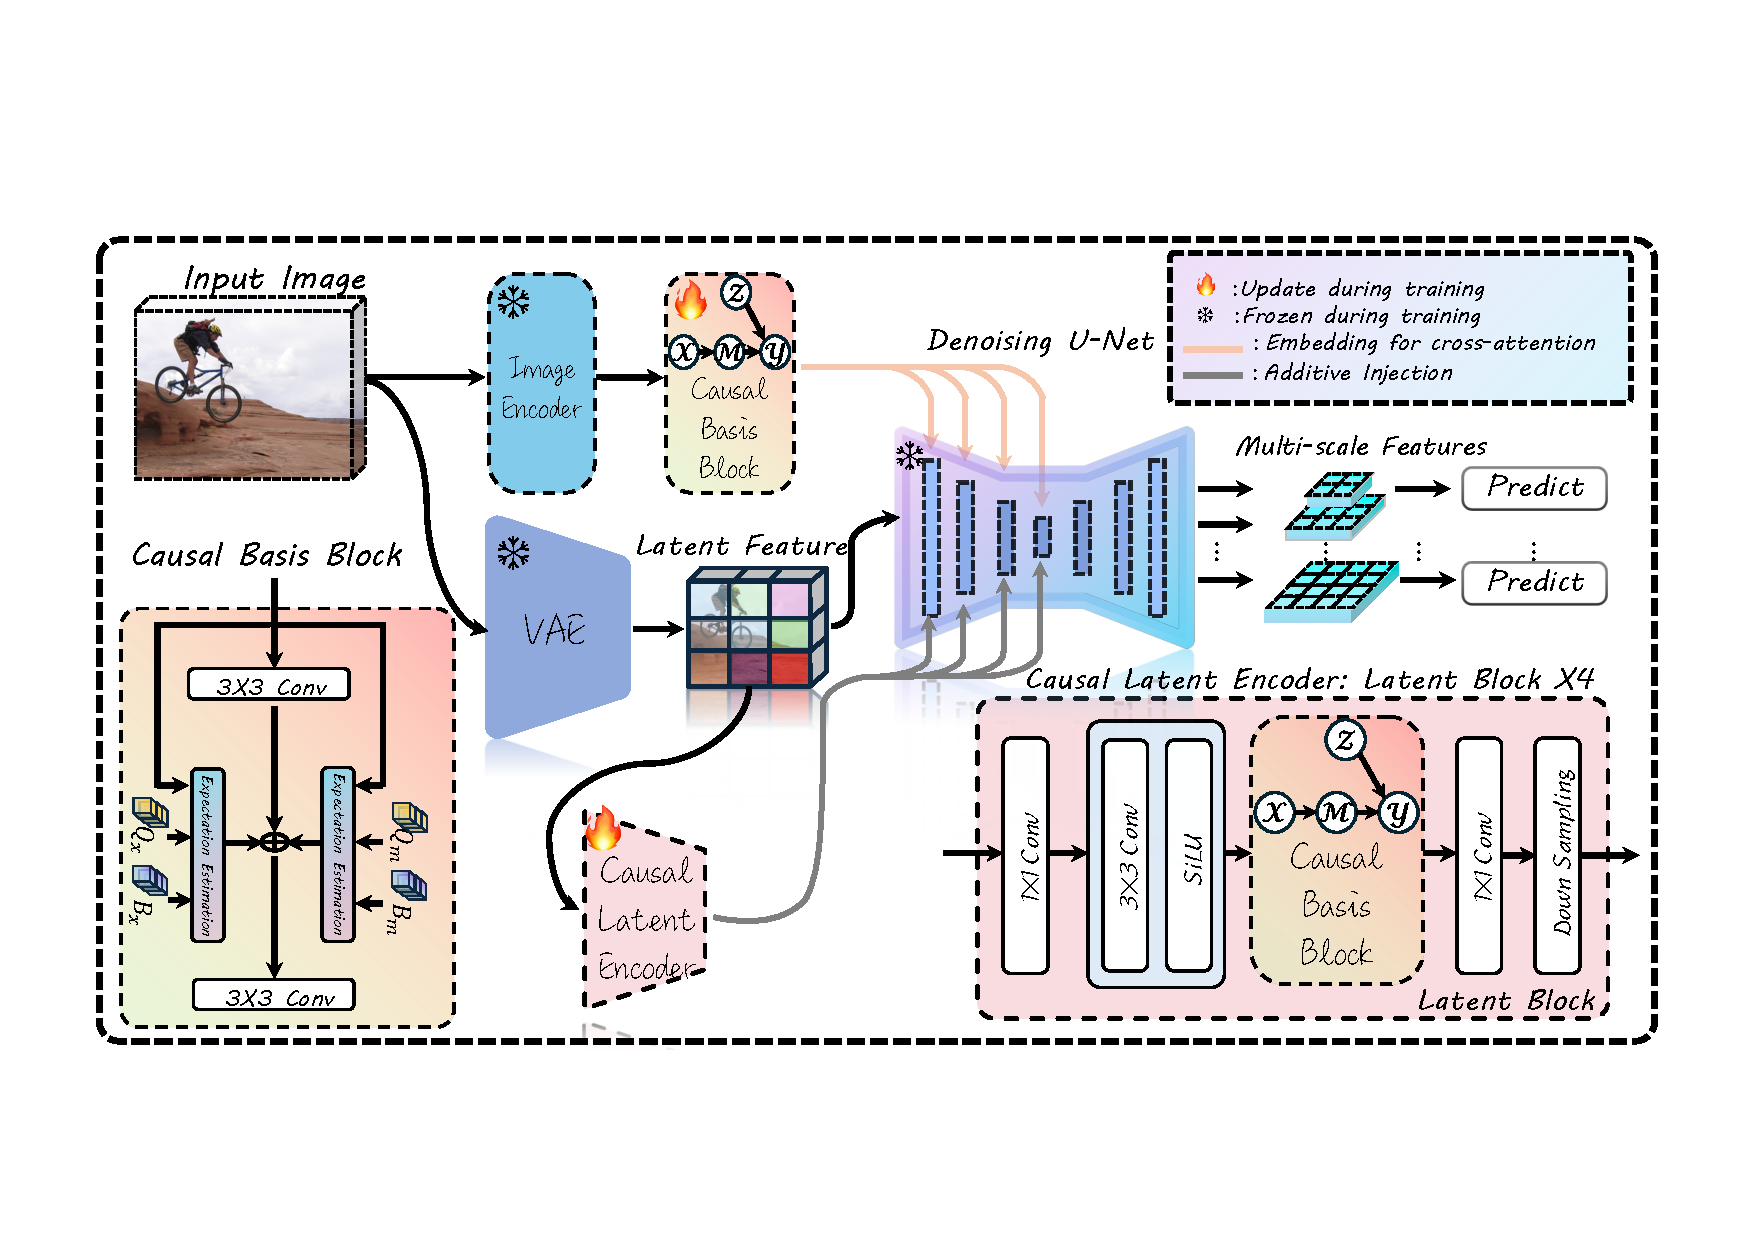
\includegraphics[width=1.00\textwidth]{supp_sec/bridge_sd.pdf}
% \caption{Overall pipeline of Generative VFM–based \textit{\textbf{Bridge}}. The image is first encoded into a latent feature by the VAE and then fed into the Denoising U-Net. We apply diffusion inversion to extract intermediate features along the denoising steps. During this process, the features produced by the Causal Latent Encoder and the Image Encoder are combined with the intermediate representations of the U-Net, thereby guiding the diffusion model to generate more robust features for downstream detection tasks.}
% \label{fig:bridge_sd}    
% \end{figure*}
\begin{table*}[t]
    \centering
    \caption{Statistics of manually annotated weather labels in the DroneVehicle dataset. 
    \textbf{BBoxes} denotes the total number of annotated objects, \textbf{Area} indicates the area of each bounding box in pixels (mean ± standard deviation), 
    and the last five columns show the number of BBoxes per object category.}
    \label{tab:weather_stats}
    \begin{tabular}{l|c|c|c|c|c|c|c|c}
        \toprule
        \textbf{Weather} & \textbf{Img} & \textbf{BBoxes} & \textbf{Area (mean ± std)} & \textbf{Car} & \textbf{Truck} & \textbf{Freight Car} & \textbf{Bus} & \textbf{Van} \\
        \midrule
        Clear & 8,881 & 132,942 & 2,830 ± 3,597 & 110,815 & 11,016 & 4,131 & 4,408 & 2,572 \\
        Dark & 13,553 & 207,535 & 2,493 ± 2,504 & 183,059 & 6,190 & 5,061 & 6,905 & 6,320 \\
        Extreme Dark & 4,965 & 85,006 & 3,079 ± 3,329 & 72,955 & 3,750 & 3,236 & 3,466 & 1,599 \\
        Foggy & 1,040 & 27,087 & 1,408 ± 1,646 & 22,950 & 1,167 & 972 & 554 & 1,444 \\
        \bottomrule
    \end{tabular}
\end{table*}

\input{supp_sec/facl.tex}
\begin{table}[t!]
\centering
\caption{DG Results (\%) on five benchmarks using ResNet101 Backbone.}
\vspace{-4pt}
\label{tab:resnet_five_datasets}
\footnotesize
\begin{tabularx}{\linewidth}{
>{\raggedright\arraybackslash}X |
>{\centering\arraybackslash}p{0.8cm} |
>{\centering\arraybackslash}p{0.8cm} |
>{\centering\arraybackslash}p{0.8cm} |
>{\centering\arraybackslash}p{0.8cm} |
>{\centering\arraybackslash}p{0.8cm}
}
\toprule
\textbf{Method} & \textbf{BDD} & \textbf{Foggy} & \textbf{DWD} & \textbf{Drone} & \textbf{R2A} \\
\midrule
ResNet101~\cite{he2016deep} & 44.0 & 47.2 & 35.9 & 31.2 & 35.5 \\
\rowcolor{lightgreen}
Ours  & \textbf{45.3} & \textbf{49.5} & \textbf{37.0} & \textbf{32.1} & \textbf{36.8} 
\\

\bottomrule

\end{tabularx}
\label{tag:resnet}
\end{table}


\begin{table}[ht]
    \centering
    \caption{Performance comparison with other methods under In-Domain and Cross-Domain settings.}
    \vspace{-4pt}
    \label{tab:performance_refined}

    {\small
    \setlength{\tabcolsep}{10pt}
    \resizebox{1\columnwidth}{!}{
    \begin{tabular}{c|c|cc}
    \toprule
    \multirow{2}{*}{\textbf{Method}} 
        & \textbf{In-Domain} 
        & \multicolumn{2}{c}{\textbf{Cross-Domain}} \\
    \cline{2-4}
        & \textbf{Cityscapes} & \textbf{BDD} & \textbf{Foggy} \\
    \midrule
    GDD~\cite{he2025generalized}& 59.8 & 50.1 & 46.6 \\
    Boost~\cite{he2025boosting} & 61.1 & 50.7 & 49.3 \\
    Ours 
        & \textbf{61.8} \textcolor{red}{(+0.7)}
        & \textbf{53.6} \textcolor{red}{(+2.9)}
        & \textbf{53.1} \textcolor{red}{(+3.8)} \\
    \bottomrule
    \end{tabular}}
    }
\label{tab:indomain}
\end{table}

\begin{table*}[t]
    \centering
    \caption{Generalization Detection Results (\%) on Cityscapes-Corruption Benchmark.}
    \vspace{-4pt}
    \label{tab:cityscapes-c}
    \setlength{\tabcolsep}{4pt}
    \renewcommand{\arraystretch}{1.0}
    \resizebox{2.1\columnwidth}{!}{%
    \begin{tabular}{l|ccc|cccc|ccc|ccccc|>{\columncolor{gray!20}}c}
    \toprule
    & \multicolumn{3}{c|}{\textbf{Noise}} & \multicolumn{4}{c|}{\textbf{Blur}} & \multicolumn{3}{c|}{\textbf{Weather}} & \multicolumn{5}{c|}{\textbf{Digital}} & \\
    \textbf{Methods} & Gauss. & Shot & Impulse & Defocus & Glass & Motion & Zoom & Snow & Frost & Fog & Bright & Contrast & Elastic & JPEG & Pixel & \textbf{mPC \textcolor{red}{$\uparrow$}} \\
    \midrule
     GDD \footnotesize{\textit{(Diff. Detector, SD)}}\normalsize~\cite{he2025generalized}  \textit{\scriptsize{(\textcolor{darkblue}{CVPR'25})}} & 20.3 & 23.2 & 17.2 & 26.8 & 21.7 & 23.7 & 3.4 & 16.6 & 24.2 & 32.5 & 34.4 & 30.6 & 33.7 & 29.1 & 24.4 & 24.1 \\
     Boost\footnotesize{ \textit{(Diff. Detector, SD)}}\normalsize~\cite{he2025boosting} \textit{\scriptsize{(\textcolor{darkblue}{ICCV'25})}}  & 23.1 & 26.6 & 20.6 & 29.7 & 24.5 & 25.5 & 4.1 & 18.3 & 28.2 & \textbf{37.2} & \textbf{39.2} & \textbf{35.5} &\textbf{37.4} & 32.7 & 28.8 & 27.4 \\ 
         \midrule
       \rowcolor{lightgreen}
       \textit{\textbf{Ours (Diff. Detector, SD)}}  & \textbf{27.3} & \textbf{29.7} & \textbf{26.4} & \textbf{30.3} & \textbf{29.4} & \textbf{27.8} & \textbf{11.5} & \textbf{23.6} & \textbf{27.3} & 34.3 & 35.7 & 33.1 & 35.0 & \textbf{33.7} & \textbf{32.2} & \textbf{29.2} \\ 
    \bottomrule
    \end{tabular}%
    }
\label{tab:city_c}
\end{table*}


\begin{figure*}[t]
    \centering
    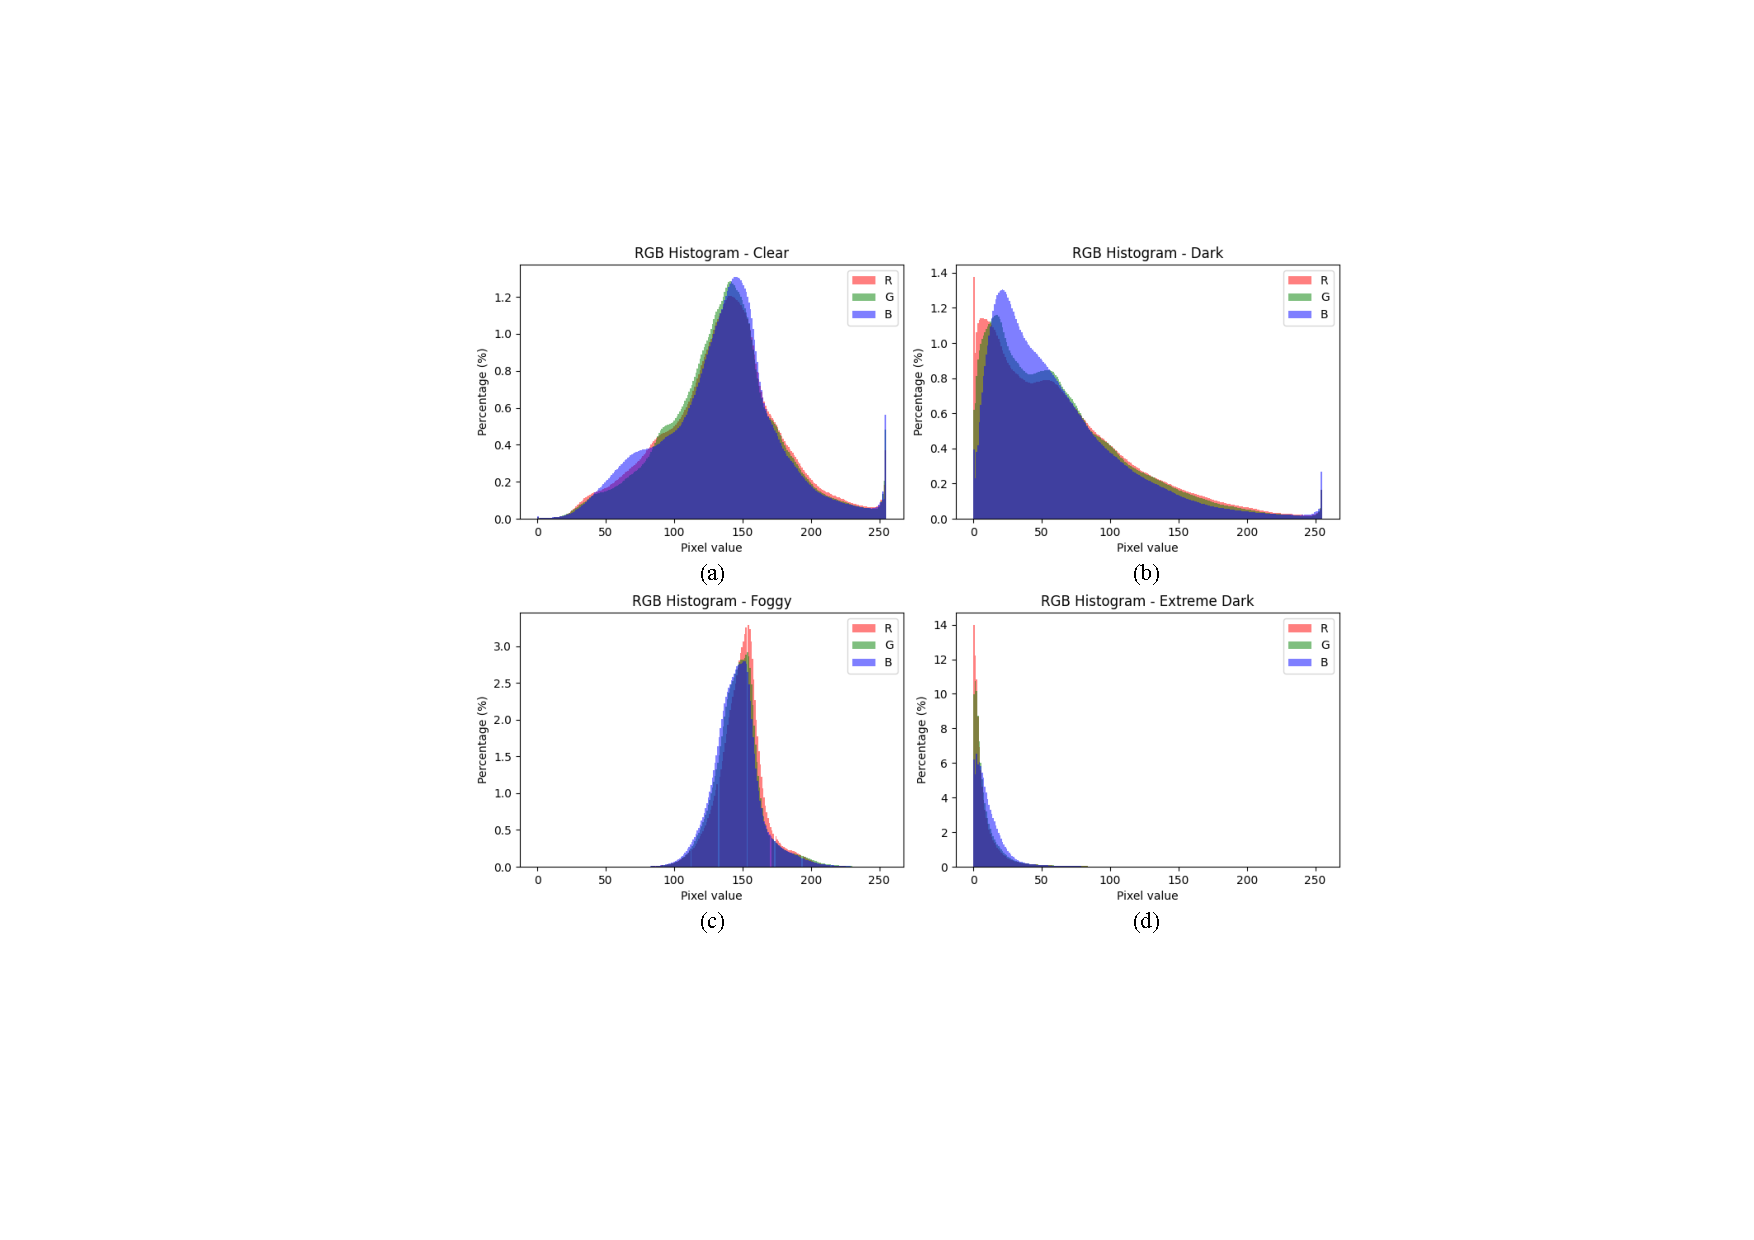
\includegraphics[width=1.0\textwidth]{supp_sec/hist_drone.pdf}
    \caption{RGB histograms under varying conditions: (a) clear (balanced), (b) low-light (left-shifted peaks), (c) foggy (high-intensity concentration), and (d) extremely dark (sharp peak near zero).}
    \label{fig:hist_drone}
\end{figure*}

\begin{figure*}[t]
    \centering
    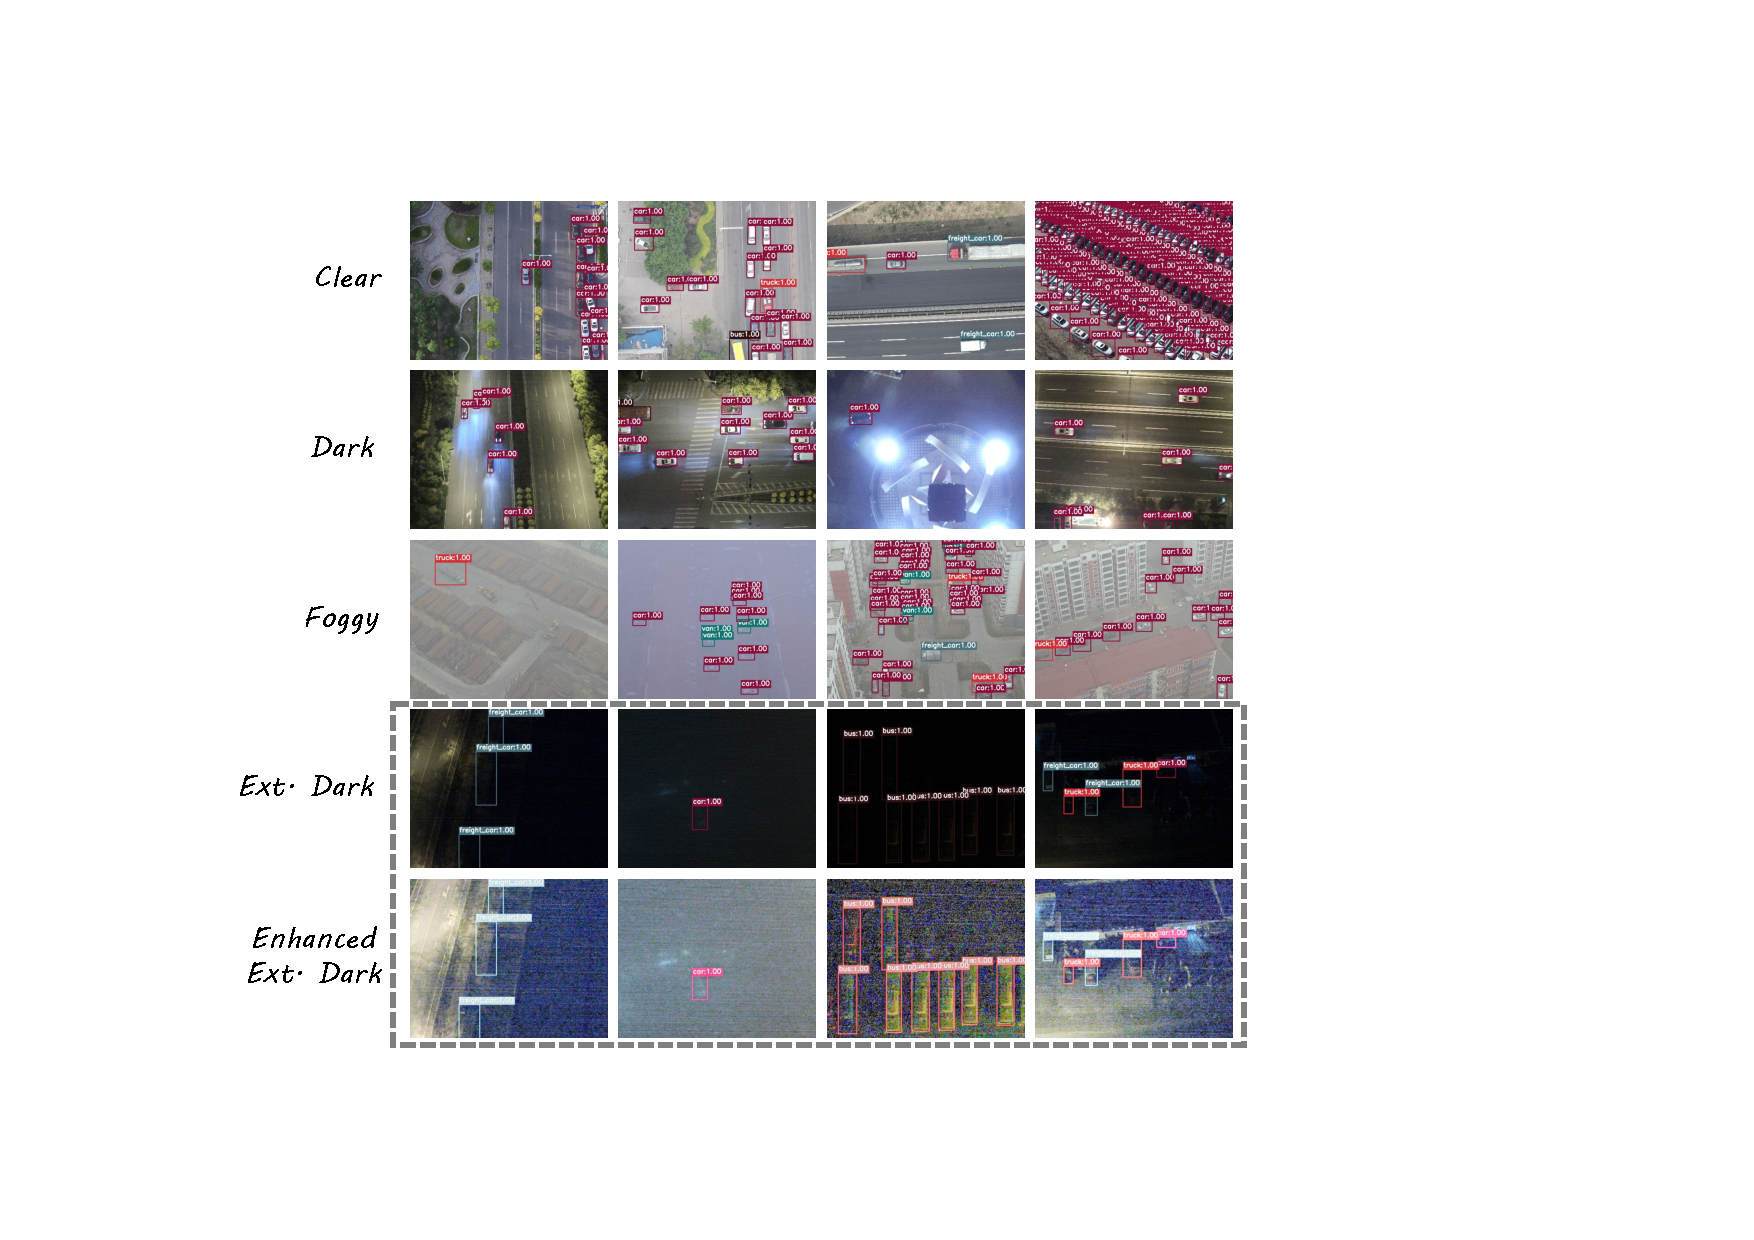
\includegraphics[width=1.0\textwidth]{supp_sec/drone_images.pdf}
    \caption{Examples of different weather conditions. The bottom row shows enhanced images generated using HVI-CIDNet~\cite{yan2025hvi}, which improve visibility for illustration purposes only.}
    \label{fig:drone_images}
    % \vspace{-6pt}
\end{figure*}

% \begin{table}[ht]
    \centering
    \caption{Ablation study of the proposed \textit{Bridge} module built upon a Generative VFM. Each row adds one component incrementally.}
    \vspace{-4pt}
    \label{tab:ablation}
    \setlength{\tabcolsep}{10pt}
    \resizebox{1\columnwidth}{!}{
    \begin{tabular}{l|cccc|>{\columncolor{gray!20}}c}
    \toprule
    \textbf{Method} & \textbf{DF} & \textbf{DR} & \textbf{NR} & \textbf{NS} & \textbf{Avg} \\
    \midrule
    \textbf{Baseline} & 45.3 & 43.3 & 26.0 & 48.4 & 40.8 \\
    \textbf{+ Image Encoder} & 46.5 & 45.9 & 28.5 & 50.7 & 42.9 \\
    \textbf{+ Latent Encoder} & 45.9 & 45.9 & 30.0 & 51.2 & 43.3 \\
    \rowcolor{lightgreen}
    \textbf{+ CBB (Full Model)} & \textbf{47.5} & \textbf{47.0} & \textbf{30.2} & \textbf{51.9} & \textbf{44.2} \\
    \bottomrule
    \end{tabular}}
\label{tab:sd_ablation}
\end{table}


% \section{Bridge for Generative VFM}
% Overall, our approach builds on the Boost~\cite{he2025boosting} architecture, with some structural differences. Figure~\ref{fig:bridge_sd} illustrates the pipeline of the Generative VFM-based \textit{\textbf{Bridge}}. The input image is processed by an \textit{Image Encoder} (CLIP) to extract high-level semantic information as a visual prompt. Compared to the manually constructed text-class prompts in Boost, the visual prompt ensures consistency between training and testing, eliminating the need for the elaborate self-distillation strategy used in Boost. Additionally, we introduce a \textit{Latent Encoder} following the T2I-Adapter~\cite{mou2024t2i} design, which injects multi-scale conditional features into the intermediate layers of the frozen Denoising U-Net via residual connections. This preserves the rich visual priors of the original generative model while guiding its feature space to adapt to downstream detection tasks. Furthermore, to mitigate spurious correlations, we embed CBB modules in both the \textit{Image Encoder} and the \textit{Latent Encoder}, generating features with reduced spurious biases through a front-door adjustment mechanism, thereby providing more robust representations for detection tasks.




% Table~\ref{tab:sd_ablation} presents the ablation study of the Generative VFM–based \textit{\textbf{Bridge}} on the Diverse Weather Dataset. As shown, introducing the \textit{Image Encoder} yields a 2.1 mAP improvement. Incorporating the latent encoder further brings a 0.4 mAP gain by leveraging multi-scale generative features to guide the diffusion model toward downstream detection tasks. Finally, adding the CBB module enables the model to learn more robust representations, leading to a final performance of 44.2 mAP. These results collectively demonstrate the effectiveness of each component in the proposed framework.






\section{Details of FACL}
In this subsection, we provide more details about the comparison between the recent state-of-the-art front-door approach and our proposed model to block confounders in detection tasks. 

GOAT~\cite{wang2024vision} FACL~\textit{\scriptsize{(\textcolor{darkblue}{CVPR'24})}}, which leverages a multi-head attention mechanism to approximate the expectation terms in the front-door formulation. Specifically, the cross-attention operation is employed to estimate the expectations over the potential input features $\boldsymbol{x}'$ and the mediator features $\boldsymbol{m}$, respectively. The overall process can be formulated as follows:
{\setlength\abovedisplayskip{0pt}
\setlength\belowdisplayskip{0pt}
\small
\begin{gather}
\mathbb{E}_{x'}[\boldsymbol{x}']\approx\sum_{x'} P(\boldsymbol{x}'|\boldsymbol{g}_1)\boldsymbol{x}'= \sum_i\frac{\text{exp}(\boldsymbol{g}_1 \boldsymbol{x}'^T_i)}{\sum_{j}\text{exp}(\boldsymbol{g}_1 \boldsymbol{x}'^T_j)} \boldsymbol{x}_i', \\
\mathbb{E}_{m|x}[\boldsymbol{m}]\approx\sum_{m} P(\boldsymbol{m}|\boldsymbol{g}_2)\boldsymbol{m}= \sum_i\frac{\text{exp}(\boldsymbol{g}_2 \boldsymbol{m}_i^T)}{\sum_{j}\text{exp}(\boldsymbol{g}_2 \boldsymbol{m}^T_j)} \boldsymbol{m}_i,
\label{eq:FA}
\end{gather}}where $\boldsymbol{g}_1$ and $\boldsymbol{g}_2$ denote the query embeddings obtained from two learnable projection functions acting on the input features $\boldsymbol{x}$.
Here, $\boldsymbol{x}'$ represents the potential input samples from the entire representation space, which are different from the current inputs $\mathcal{X} = \boldsymbol{x}$, and are used to construct the cross-sampling expectation term in the front-door adjustment.
The attention weights $P(\boldsymbol{x}'|\boldsymbol{g}_1)$ and $P(\boldsymbol{m}|\boldsymbol{g}_2)$ correspond to the normalized similarity scores between the query and key features, allowing the model to approximate the in-sampling and cross-sampling expectations through the attention mechanism.

However, directly sampling $\boldsymbol{x}'$ from the entire training set via K-means clustering is almost infeasible for dense prediction tasks. The clustering space is extremely high-dimensional, containing an enormous number of feature instances with continuous distributions and lacking semantic consistency across local regions. Therefore, we apply \textit{dropout} to intervene on $\boldsymbol{x}$ and obtain $\boldsymbol{x}'$. The stochastic masking introduced by dropout acts as an \textit{intervention} operator on the features. Table~\ref{tab:map_five_datasets} reports the DG results on five benchmark datasets. While the dropout-based FACL~\cite{wang2024vision} improves over the baseline, our method still consistently achieves higher performance across all datasets, particularly on dense prediction tasks such as DWD and Drone.

\section{Additional Ablation Study}


In addition to VFMs, we also evaluate our \textbf{\textit{Bridge}} framework on a classic backbone, ResNet-101, to further verify its generalization ability and robustness. Table~\ref{tab:resnet_five_datasets} reports the results on five DG benchmarks. As shown, \textbf{\textit{Bridge}} consistently improves performance over the ResNet-101 across all datasets, with gains of +1.3\% on BDD, +2.3\% on Foggy, +1.1\% on DWD, +0.9\% on Drone, and +1.3\% on R2A, demonstrating that our \textbf{\textit{Bridge}} framework is effective not only with VFMs but also with classic backbones like ResNet-101 across diverse domain shifts.


\section{Additional Quantitative Experiments}

Table~\ref{tab:indomain} shows the model’s performance on in-domain testing using the Cityscapes benchmark. It can be observed that, although our method improves in-domain performance by only 0.7 mAP, it achieves significant gains of \textbf{2.9} and \textbf{3.8} mAP in \textbf{cross-domain tests}. This further demonstrates the strong generalization ability of the \textbf{\textit{Bridge}} across different domains.

In addition to the five DG benchmarks evaluated in the manuscript, we further follow the OADG~\cite{lee2024object} setting, evaluating our method on Cityscapes-C~\cite{michaelis2019benchmarking} with 15 corruption types. Table~\ref{tab:city_c} presents the detailed metrics under different corruptions, where our \textbf{\textit{Bridge}} achieves state-of-the-art performance.


% \section{Explanation of Intervention: Do-Operator}

% In causal inference, the \emph{do-operator}, denoted as $do(X = x)$, was described by \citet{pearl2016causal} as a formal way to represent \emph{intervention} within causal reasoning.


% In observational data, for discriminative models, we typically compute the conditional probability
% \begin{equation}
% P(Y \mid X = x),
% \end{equation}
% which represents the likelihood of \( Y \) given the observed value of \( X \).


% However, this probability may not reflect a causal relationship between \(X\) and \(Y\), as \(X\) may be correlated with \(Y\) due to the influence of confounding variables.


% In contrast, the do-operator expresses an explicit intervention:
% \begin{equation}
% P(Y \mid do(X = x)),
% \end{equation}
% which denotes the distribution of \(Y\) when the variable \(X\) is actively set to the value \(x\) through an external intervention, rather than being passively observed.


\section{Instability of \texorpdfstring{$\mathcal{P}(\mathcal{Z}\mid \mathcal{X})$}{P(Z|X)}}
As mentioned in Section 3.1.2 of the manuscript, in this section, we explain why $\mathcal{P}(\mathcal{Z}\mid\mathcal{X})$ becomes unstable under limited sample settings.
\begin{theorem}[Instability of $\mathcal{P}(\mathcal{Z}\mid \mathcal{X})$ under finite samples]
Consider a fixed input $\mathcal{X} = x$, and let the confounder $\mathcal{Z}$ take finitely many values 
$\{z_1, \dots, z_K\}$. 
Assume that $\mathcal{X}$ and $\mathcal{Z}$ are independent, so that the true conditional probabilities are uniform:
\[
p_k := \mathcal{P}(\mathcal{Z} = z_k \mid \mathcal{X} = x) = \frac{1}{K}, \quad k = 1, \dots, K.
\]
Assume we observe $n$ independent samples $\{\mathcal{Z}_i\}_{i=1}^n$ drawn from 
$\mathcal{P}(\mathcal{Z} \mid \mathcal{X} = x)$. 
Define the empirical frequency
\[
\hat p_k := \frac{1}{n}\sum_{i=1}^n \mathbf{1}\{\mathcal{Z}_i = z_k\}.
\]
Then, for any $\delta > 0$,
\[
\mathcal{P}\!\left(\hat p_k - p_k \ge \delta\right) \le \exp\!\left(-2n\delta^2\right).
\]
\end{theorem}

\begin{proof}\renewcommand{\qedsymbol}{}
For the fixed $k$, define indicator random variables 
$X_i^{(k)} := \mathbf{1}\{\mathcal{Z}_i = z_k\}$. 
Each $X_i^{(k)}$ is independent and bounded in $[0,1]$, 
with expectation $\mathbb{E}[X_i^{(k)}] = p_k = 1/K$. 
Hence,
\[
\hat p_k = \frac{1}{n}\sum_{i=1}^n X_i^{(k)}.
\]

By Hoeffding's inequality~\cite{hoeffding1963probability} for bounded independent variables,
\[
\mathcal{P}\!\left(\hat p_k - p_k \ge \delta\right)
\le \exp\!\left(-2n\delta^2\right),
\]
which completes the proof.
\end{proof}

\noindent
\textbf{Discussion.}  
Although theoretically $\mathcal{X}$ and $\mathcal{Z}$ are independent and all $p_k$ are equal to $1/K$, 
finite sample fluctuations can make the empirical $\hat{p}_k$ deviate significantly from $p_k$. 
In particular, small $n$ allows some $\hat p_k$ to be temporarily overestimated, 
which can cause the mixture
\begin{equation}
    \mathcal{P}(\mathcal{Y} \mid \mathcal{X}) 
    = \sum_{\mathcal{Z}} \mathcal{P}(\mathcal{Y} \mid \mathcal{X}, \mathcal{Z}) \, \mathcal{P}(\mathcal{Z} \mid \mathcal{X}) ,
    \label{equ:bayes_rule}
\end{equation}
to be dominated by one confounder component purely due to sampling noise, not any causal effect of $\mathcal{X}$ on $\mathcal{Z}$.






% \clearpage


{
    \small
    \bibliographystyle{ieeenat_fullname}
    \bibliography{main}
}

\end{document}
